\documentclass[aspectratio=169,11pt]{beamer}

% ================================================================
% "TABIIY TILNI QAYTA ISHLASH" KURSI
% MA'RUZA 2 --- Klassik usullar bilan matnlarni tasniflash,
%               klassifikator modellarni baholash va NLPdagi etika
%              (d02_klassik_tasnif.tex)
% Arxetiplar: [A][B][C][D][E] + 4 tsikl [F][G][H][I][J][K][L] +
%             [M][N][O][P][Q][R] + ilova [S]
% Rendered slayd soni: ~43  (L2 uchun ruxsat etilgan istisno: 40-44)
% ================================================================

% ================================================================
% RANGLAR  (asl fayldan o'zgarishsiz)
% ================================================================
\definecolor{cnublue}{rgb}{0.07,0.14,0.62}
\definecolor{cnubluelight}{rgb}{0.18,0.30,0.72}
\definecolor{cnubluebg}{rgb}{0.90,0.92,0.97}
\definecolor{deepblue}{rgb}{0.07,0.14,0.62}
\definecolor{deepred}{rgb}{0.60,0.00,0.00}
\definecolor{deepgreen}{rgb}{0.00,0.45,0.00}
\definecolor{halfgray}{gray}{0.55}

% ================================================================
% BEAMER MAVZU --- Boadilla + maxsus footer  (asl fayldan o'zgarishsiz)
% ================================================================
\usetheme{Boadilla}

\setbeamercolor{structure}{fg=cnublue}
\setbeamercolor{frametitle}{bg=cnublue,fg=white}
\setbeamercolor{title}{bg=cnublue,fg=white}
\setbeamercolor{block title}{bg=cnublue,fg=white}
\setbeamercolor{block body}{bg=cnubluebg,fg=black}
\setbeamercolor{alerted text}{fg=deepred}
\setbeamercolor{author in head/foot}{bg=cnubluelight,fg=white}
\setbeamercolor{section in head/foot}{bg=cnublue,fg=white}
\setbeamercolor{page number in head/foot}{bg=cnubluelight,fg=white}

\setbeamertemplate{mini frame}{}
\setbeamertemplate{mini frame in current section}{}
\setbeamertemplate{mini frame in current subsection}{}
\setbeamertemplate{headline}{}
\setbeamertemplate{navigation symbols}{}

\setbeamertemplate{footline}{%
  \leavevmode%
  \hbox{%
    \begin{beamercolorbox}[wd=0.17\paperwidth,ht=2.5ex,dp=1.25ex,leftskip=0.5em]{author in head/foot}%
      \usebeamerfont{author in head/foot}\scriptsize\insertshortauthor%
    \end{beamercolorbox}%
    \begin{beamercolorbox}[wd=0.69\paperwidth,ht=2.5ex,dp=1.25ex,center]{section in head/foot}%
      \usebeamerfont{section in head/foot}%
      \scriptsize\insertsectionnavigationhorizontal{0.69\paperwidth}{}{}%
    \end{beamercolorbox}%
    \begin{beamercolorbox}[wd=0.14\paperwidth,ht=2.5ex,dp=1.25ex,rightskip=0.5em]{page number in head/foot}%
      \hfill\scriptsize\color{white}%
      \insertframenumber{}/\inserttotalframenumber%
    \end{beamercolorbox}%
  }%
  \vskip0pt%
}

% ================================================================
% PAKETLAR  (asl fayldan o'zgarishsiz)
% ================================================================
\usepackage[utf8]{inputenc}
\usepackage[T1]{fontenc}
\usepackage{lmodern}
\usepackage{amsmath,amssymb}
\usepackage{booktabs}
\usepackage{xcolor}
\usepackage{listings}
\lstset{
    language=Python,
    basicstyle=\ttfamily\scriptsize,
    keywordstyle=\bfseries\color{deepblue},
    emphstyle=\ttfamily\color{deepred},
    stringstyle=\color{deepgreen},
    commentstyle=\itshape\color{halfgray},
    numbers=left,
    numberstyle=\scriptsize\color{halfgray},
    rulesepcolor=\color{cnublue!30},
    frame=shadowbox,
    breaklines=true,
    showstringspaces=false,
    tabsize=2
}
\usepackage{tcolorbox}
\tcbuselibrary{skins}
\tcbset{
  defbox/.style={colback=cnubluebg,colframe=cnublue,
                 fonttitle=\small\bfseries\color{white},
                 attach boxed title to top left={yshift=-2mm,xshift=4mm},
                 boxed title style={colback=cnublue,colframe=cnublue}},
  warnbox/.style={colback=orange!8,colframe=orange!70!black,
                  fonttitle=\small\bfseries},
  okbox/.style={colback=green!7,colframe=green!55!black,
                fonttitle=\small\bfseries}
}
\usepackage{tikz}
\usetikzlibrary{arrows.meta,positioning}

% ================================================================
% QO'SHIMCHALAR  (asl fayldan o'zgarishsiz)
% ================================================================
\AtBeginSection[]{%
  \begin{frame}{Qayerdamiz?}
    \tableofcontents[currentsection]
  \end{frame}}

\newcommand{\bunda}[1]{{\small\textbf{bunda:}\; #1}}
\newcommand{\bajarildi}{{\color{deepgreen}\large$\checkmark$}\;}

% ================================================================
% METAMA'LUMOT
% ================================================================
\title[Klassik Tasnif]{Klassik Usullar bilan Matnlarni Tasniflash}
\subtitle{Tabiiy tilni qayta ishlash --- 2-ma'ruza}
\author[A.A.\,Abdulali]{A.A.\,Abdulali}
\date{16-iyun 2026}
\institute{11:00--12:20 \quad$\cdot$\quad VMQ 425-son, mavzu \textnumero{}2}

% ================================================================
\begin{document}
% ================================================================

% ----------------------------------------------------------------
% [A] TITUL
% ----------------------------------------------------------------
\maketitle

% ================================================================
\section[Kirish]{Kirish: Vektordan Sinfgacha}
% ================================================================

% ----------------------------------------------------------------
% [B] TAKRORLASH: L1 dan ikki savol
% ----------------------------------------------------------------
\begin{frame}{Takrorlash: L1 Natijalarini Tekshiramiz}
  \begin{columns}[T]
    \begin{column}{0.49\textwidth}
      \begin{tcolorbox}[warnbox,title=Savol 1]
        \small
        $D_1{=}$``nlp qiziq'',\; $D_2{=}$``python foydali'',\;
        $D_3{=}$``nlp foydali''\\[3pt]
        $\mathrm{TF\text{-}IDF}(\text{qiziq},\,D_1) = ?$\\
        \footnotesize [$\mathrm{df}=1$,\; $N=3$,\; $\mathrm{TF}=1$]
      \end{tcolorbox}
    \end{column}
    \begin{column}{0.49\textwidth}
      \begin{tcolorbox}[warnbox,title=Savol 2]
        \small
        BoW vektori $[1,\,1,\,0,\,0]$ nima
        \textbf{saqlaydi}?\; Nima \textbf{yo'qoladi}?
      \end{tcolorbox}
    \end{column}
  \end{columns}
  \pause
  \vspace{4pt}
  \begin{columns}[T]
    \begin{column}{0.49\textwidth}
      \begin{tcolorbox}[okbox,title=Javob 1]
        \small
        $\mathrm{IDF}=\ln(3/1)\approx 1.099$\\
        $\mathrm{TF\text{-}IDF}=1\times 1.099=\mathbf{1.099}$\\
        \footnotesize\textcolor{halfgray}{P1 assert: \texttt{abs(v-1.099)<1e-3}}
      \end{tcolorbox}
    \end{column}
    \begin{column}{0.49\textwidth}
      \begin{tcolorbox}[okbox,title=Javob 2]
        \small
        Saqlaydi: so'zlar \textbf{chastotasi}.\\
        Yo'qoladi: so'z \textbf{tartibi} (word order).\\
        \footnotesize\textcolor{halfgray}{Bugun: shu vektorda tasniflash qilamiz.}
      \end{tcolorbox}
    \end{column}
  \end{columns}
\end{frame}

% ----------------------------------------------------------------
% [C] MAQSADLAR
% ----------------------------------------------------------------
\begin{frame}{Bugungi Maqsadlar}
  \begin{enumerate}\setlength{\itemsep}{7pt}
    \item \textbf{Keltirib chiqara olasiz:} LR gradient ---
          $\sigma(z)\!\to\!\ell_i\!\to\!L\!\to\!\partial L/\partial w_j$ ---
          uch qadamda.
    \item \textbf{Hisoblaya olasiz:} Naive Bayes posterior nisbatini
          Laplace bilan (qo'lda misol: nisbat$=3.375$).
    \item \textbf{Qurasiz:} confusion matrix dan accuracy, precision,
          recall, $F_1$ beshta raqam ustida.
    \item \textbf{Tanqidiy baho bera olasiz:} sentiment klassifikatorida
          kamida uch etika muammosini aniqlay olasiz.
  \end{enumerate}
  \vspace{5pt}
  \begin{tcolorbox}[defbox,title=Oldingi bilimlar]
    \small
    TF-IDF vektori (L1);\; Python funksiyalar;\;
    $\exp(\cdot)$ va $\ln(\cdot)$ tushunchasi.
  \end{tcolorbox}
\end{frame}

% ----------------------------------------------------------------
% [D] REJA
% ----------------------------------------------------------------
\begin{frame}{Dars Rejasi: To'rt Tsikl}
  \begin{center}
    \small
    \begin{tabular}{clr}
      \toprule
      Tsikl & Mavzu & Vaqt \\
      \midrule
      1 & Logistik regressiya: sigmoid $\to$ gradient & 22 daq \\
      2 & Naive Bayes: Bayes teoremi + Laplace silliqlash & 25 daq \\
      3 & Metrikalar: confusion matrix, precision, recall, $F_1$ & 20 daq \\
      4 & NLPda etika: uch muammo, oqibatlar & 10 daq \\
      \midrule
        & Xulosa va P2 ko'prigi & 3 daq \\
      \bottomrule
    \end{tabular}
  \end{center}
  \vspace{4pt}
  \small\textcolor{halfgray}{Barcha misollar: o'zbek matni, CPU,
  Kaggle bepul rejimi (T4/P100 shart emas).}
\end{frame}

% ----------------------------------------------------------------
% [E] MUAMMO: TF-IDF vektori bor lekin sinf yo'q
% ----------------------------------------------------------------
\begin{frame}{Muammo: Vektori Bor --- Sinfi Yo'q}
  \begin{columns}[T]
    \begin{column}{0.52\textwidth}
      \small
      \textbf{Vaziyat (L1 dan davom):}\\[4pt]
      Sharh: ``Sifati \textbf{yaxshi}, ammo
      yetkazib berish \textbf{past} edi.''\\[5pt]
      TF-IDF (fragment):\\[2pt]
      \begin{tcolorbox}[warnbox]
        \footnotesize
        yaxshi:\;0.51\quad past:\;0.38\quad
        sifat:\;0.44\quad ammo:\;0.22
      \end{tcolorbox}
      \vspace{5pt}
      \textbf{Soda qoida:} ``yaxshi'' bor $\Rightarrow$ musbat?\\
      \alert{Xato!} ``ammo past'' kontrastni ko'rmaydi.
    \end{column}
    \begin{column}{0.44\textwidth}
      \vspace{8pt}
      \begin{tcolorbox}[defbox,title=NLP yondashuvi]
        \small
        TF-IDF vektor $\mathbf{x}$\\[2pt]
        $\downarrow$\\[2pt]
        \textbf{Matematik model}\\[2pt]
        $\downarrow$\\[2pt]
        $P(\text{musbat}\mid\mathbf{x})$\\[2pt]
        $\downarrow$\\[2pt]
        Qaror ($>\!0.5$ ?)
      \end{tcolorbox}
      \vspace{5pt}
      \small Bugun ikkita model:\\
      \quad 1.\ Logistik regressiya\\
      \quad 2.\ Naive Bayes
    \end{column}
  \end{columns}
\end{frame}

% ================================================================
\section[Log.\ Reg.]{Logistik Regressiya}
% ================================================================

% ----------------------------------------------------------------
% [F1] INTUITSIYA: ehtimollikka asoslangan qaror
% ----------------------------------------------------------------
\begin{frame}{Logistik Regressiya --- Nima Uchun Ehtimollik?}
  \begin{columns}[T]
    \begin{column}{0.50\textwidth}
      \small
      \textbf{``Ikkali qiymat'' yetarli emas:}\\[5pt]
      \begin{tabular}{@{}p{4.5cm}l@{}}
        ``Zo'r mahsulot!'' & musbat \\[2pt]
        ``Mahsulot yaxshi ammo\ldots'' & noaniq? \\[2pt]
        ``Yomon edi.'' & salbiy \\
      \end{tabular}
      \vspace{6pt}\\
      Model ikkinchi qatordagi
      \textbf{noaniqlikni} ifodalashi kerak.
    \end{column}
    \begin{column}{0.47\textwidth}
      \begin{tcolorbox}[defbox,title=Ehtimollik beradi]
        \small
        $P(\text{musbat})=0.95$ --- ishonchli\\[2pt]
        $P(\text{musbat})=0.53$ --- noaniq\\[2pt]
        $P(\text{musbat})=0.08$ --- salbiy\\[4pt]
        \textbf{Ostonani moslashtirish:}\\
        spam filtri: $>\!0.90$\\
        tibbiy diagnoz: $>\!0.30$
      \end{tcolorbox}
    \end{column}
  \end{columns}
\end{frame}

% ----------------------------------------------------------------
% [G1] RASMIY TA'RIF: sigmoid + bunda
% ----------------------------------------------------------------
\begin{frame}{Logistik Regressiya: Rasmiy Ta'rif}
  \begin{tcolorbox}[defbox,title=Ta'rif: LR Bashorat Funksiyasi]
    \[
      P(y{=}1\mid\mathbf{x})
      \;=\;
      \sigma(\mathbf{w}\cdot\mathbf{x}+b)
      \;=\;
      \frac{1}{1+e^{-(\mathbf{w}\cdot\mathbf{x}+b)}}
    \]
  \end{tcolorbox}
  \vspace{3pt}
  \bunda{%
    $\mathbf{x}$ = kirish vektori (TF-IDF);\;
    $\mathbf{w}$ = og'irliklar (o'rganiladi);\;
    $b$ = bias;\;
    $\sigma$ = sigmoid;\;
    $y{=}1$ = musbat sinf%
  }
  \vspace{5pt}
  \begin{columns}[T]
    \begin{column}{0.48\textwidth}
      \small
      \textbf{Xossalar:}
      \begin{itemize}
        \item $\sigma(z)\in(0,1)$ --- har doim ehtimollik
        \item $\sigma(0)=0.5$ --- qaror chegarasi
        \item $w_j>0$: $j$-so'z musbat tomonga ``itaradi''
        \item $w_j<0$: salbiy tomonga
      \end{itemize}
    \end{column}
    \begin{column}{0.48\textwidth}
      \small
      \textbf{Misol (ikkita so'z):}\\[3pt]
      $w_{\text{yaxshi}}=+0.8$ --- musbat signal\\
      $w_{\text{yomon}}=-1.2$ --- salbiy signal\\
      $b=-0.3$ --- boshlang'ich noaniqlik\\[4pt]
      \textcolor{halfgray}{\footnotesize Qaror:
      $\sigma(\mathbf{w}\cdot\mathbf{x}+b)>0.5$?}
    \end{column}
  \end{columns}
\end{frame}

% ----------------------------------------------------------------
% [H1a] CHIQARUV 1: model -> log-likelihood -> loss
% ----------------------------------------------------------------
\begin{frame}{LR Chiqaruvi, 1-qism: Zarar Funksiyasi}
  \small
  \textbf{1-qadam.} Bitta namuna ehtimolligi ($z_i=\mathbf{w}\cdot\mathbf{x}_i+b$):
  \[
    P(y_i\mid\mathbf{x}_i)
    = \sigma(z_i)^{y_i}\,(1-\sigma(z_i))^{1-y_i}
  \]
  \textcolor{halfgray}{\footnotesize
    ($y_i{=}1$: $\sigma(z_i)^1$;\quad $y_i{=}0$: $(1-\sigma(z_i))^1$)}
  \pause
  \textbf{2-qadam.} $N$ namuna uchun log-likelihood:
  \[
    \ell(\mathbf{w},b)
    =\sum_{i=1}^{N}
    \bigl[y_i\ln\sigma(z_i)+(1-y_i)\ln(1-\sigma(z_i))\bigr]
  \]
  \textcolor{halfgray}{\footnotesize
    (log: ko'paytma $\to$ yig'indi; underflow yo'q)}
  \pause
  \textbf{3-qadam.} Cross-entropy loss (minimizatsiya uchun):
  \[
    L(\mathbf{w},b) = -\,\frac{1}{N}\,\ell(\mathbf{w},b)
  \]
  \textcolor{halfgray}{\footnotesize
    ($\max\ell \Leftrightarrow \min L$; manfiy ishora standart konvensiya)}
\end{frame}

% ----------------------------------------------------------------
% [H1b] CHIQARUV 2: gradient -> yangilash
% ----------------------------------------------------------------
\begin{frame}{LR Chiqaruvi, 2-qism: Gradient va Yangilash Qoidasi}
  \small
  \textbf{4-qadam.} $\sigma'(z)=\sigma(z)(1-\sigma(z))$ dan foydalanib:
  \[
    \frac{\partial L}{\partial w_j}
    \;=\;
    \frac{1}{N}\sum_{i=1}^{N}\bigl(\sigma(z_i)-y_i\bigr)\,x_{ij}
  \]
  \textcolor{halfgray}{\footnotesize
    intuitiv o'qilish: ``bashorat xatosi'' $\times$ ``$j$-feature''}
  \pause
  \textbf{5-qadam.} SGD yangilash ($\alpha$ = o'rganish tezligi):
  \[
    w_j \;\leftarrow\; w_j
    - \alpha\;\frac{\partial L}{\partial w_j}
  \]
  \vspace{3pt}
  \begin{tcolorbox}[okbox,title=Mantiq]
    \small
    Agar $\sigma(z_i)>y_i$ (ortiqcha musbat bashorat)
    $\Rightarrow$ gradient $>0$
    $\Rightarrow$ $w_j$ kamayadi.\\[3pt]
    Agar $\sigma(z_i)<y_i$ (kam bashorat)
    $\Rightarrow$ gradient $<0$
    $\Rightarrow$ $w_j$ oshadi.
  \end{tcolorbox}
\end{frame}

% ----------------------------------------------------------------
% [I1] QO'LDA MISOL: LR forward pass
% ----------------------------------------------------------------
\begin{frame}{LR Qo'lda Hisob: Bitta So'rov Uchun}
  \small
  $\mathbf{x}=[\mathrm{TF\text{-}IDF(yaxshi)}{=}1.0,\;
  \mathrm{TF\text{-}IDF(yomon)}{=}0.0]$;\quad
  $\mathbf{w}=[0.8,\;{-}1.2]$,\; $b=-0.3$
  \vspace{5pt}
  \begin{columns}[T]
    \begin{column}{0.50\textwidth}
      \begin{tcolorbox}[defbox,title=Forward pass]
        \small
        $z = 0.8(1.0)+(-1.2)(0.0)+(-0.3) = 0.5$\\[5pt]
        $\sigma(0.5)=\dfrac{1}{1+e^{-0.5}}
        \approx\dfrac{1}{1.607}\approx 0.622$\\[5pt]
        $0.622>0.5$
        $\Rightarrow$ \textcolor{deepgreen}{\textbf{musbat}} \checkmark
      \end{tcolorbox}
    \end{column}
    \begin{column}{0.47\textwidth}
      \begin{tcolorbox}[defbox,title=Bitta namuna zarari ($y{=}1$)]
        \small
        $L_i = -\ln(0.622)\approx 0.475$\\[5pt]
        \textcolor{halfgray}{\footnotesize
          Noto'g'ri bashorat: $L_i$ oshadi.\\
          To'g'ri va ishonchli: $L_i$ kamayadi.}
      \end{tcolorbox}
    \end{column}
  \end{columns}
  \vspace{5pt}
  \textcolor{halfgray}{\footnotesize
    Eslatma: $e^{-0.5}\approx 0.607$;\quad
    dasturda \texttt{from scipy.special import expit; expit(0.5)}.}
\end{frame}

% ----------------------------------------------------------------
% [J1] SIZNING VAZIFANGIZ: LR
% ----------------------------------------------------------------
\begin{frame}{Sizning Vazifangiz: LR Ehtimolligi}
  \begin{tcolorbox}[warnbox,title=Vazifa (3 daqiqa)]
    \small
    Xuddi shu parametrlar:
    $\mathbf{w}=[0.8,\;{-}1.2]$,\; $b=-0.3$.\\[4pt]
    Yangi so'rov: $\mathbf{x}=[0,\;1]$
    \quad (faqat ``yomon'' so'zi uchraydi).\\[4pt]
    a)\; $z = ?$\qquad
    b)\; $\sigma(z)\approx ?$\quad ($e^{1.5}\approx 4.48$)\qquad
    c)\; Bashorat?
  \end{tcolorbox}
  \pause
  \begin{tcolorbox}[okbox,title=Javob]
    \small
    a)\; $z = 0.8(0)+(-1.2)(1)+(-0.3) = -1.5$\\[4pt]
    b)\; $\sigma(-1.5)=\dfrac{1}{1+e^{1.5}}
         \approx\dfrac{1}{5.48}\approx 0.182$\\[4pt]
    c)\; $0.182<0.5$
         $\Rightarrow$ \textcolor{deepred}{\textbf{salbiy}} \checkmark\quad
         \textcolor{halfgray}{\footnotesize
           (``yomon'' so'zi salbiy og'irlikka ega: $w_2=-1.2$)}
  \end{tcolorbox}
\end{frame}

% ----------------------------------------------------------------
% [K1] KOD <-> FORMULA: LogisticRegression  [fragile: lstlisting]
% ----------------------------------------------------------------
\begin{frame}[fragile]{LR Kodi --- Formulaga Ko'prik}
  \begin{columns}[T]
    \begin{column}{0.58\textwidth}
\begin{lstlisting}
from sklearn.pipeline import Pipeline
from sklearn.feature_extraction.text import (
    TfidfVectorizer)
from sklearn.linear_model import LogisticRegression

texts  = ["yaxshi mahsulot",
          "ajoyib sifat",
          "yomon yetkazish"]
labels = [1, 1, 0]

pipe = Pipeline([
    ('tfidf', TfidfVectorizer()),
    ('lr',   LogisticRegression(
                C=1.0,        # 1/regularizatsiya
                max_iter=200)),
])
pipe.fit(texts, labels)
p = pipe.predict_proba(["yaxshi mahsulot"])[0][1]
print(f"P(musbat) = {p:.3f}")
\end{lstlisting}
    \end{column}
    \begin{column}{0.39\textwidth}
      \small
      \begin{tabular}{@{}ll@{}}
        \toprule
        Kod & Formula \\
        \midrule
        \texttt{TfidfVectorizer} & $\mathbf{x}$ \\
        \texttt{C=1.0}           & $1/\lambda$ \\
        \texttt{max\_iter}       & epoch soni \\
        \texttt{predict\_proba}  & $\sigma(\mathbf{w}\cdot\mathbf{x}+b)$ \\
        \texttt{predict}         & $>0.5$? \\
        \bottomrule
      \end{tabular}
      \vspace{6pt}\\
      \small\textbf{Muhim:}\\
      \texttt{C} kichik $\Rightarrow$\\
      ko'proq regularizatsiya\\
      (og'irliklar kichrayadi)
    \end{column}
  \end{columns}
\end{frame}

% ----------------------------------------------------------------
% [L1] TUZOG': tengsiz ma'lumot
% ----------------------------------------------------------------
\begin{frame}{LR Tuzog'i: Tengsiz Ma'lumot (Imbalanced)}
  \begin{tcolorbox}[warnbox,title=Muammo]
    \small
    Training: 900 salbiy, 100 musbat sharh.\\
    Oddiy LR: ``hammasi salbiy'' bashorat qiladi.\\
    Natija: \texttt{accuracy=90\%} lekin \texttt{F1=0\%}
    --- butunlay foydasiz!
  \end{tcolorbox}
  \vspace{6pt}
  \begin{tcolorbox}[okbox,title=Yechim: \texttt{class\_weight=`balanced'}]
    \small
    \texttt{LogisticRegression(class\_weight='balanced')}\\[5pt]
    Avtomatik og'irlik:\quad
    $w_{\text{sinf}} = \dfrac{N}{N_{\text{sinf}}\times n_{\text{sinf}}}$\\[4pt]
    \textcolor{halfgray}{\footnotesize
      Kamroq uchraydigan sinfga ko'proq og'irlik $\Rightarrow$
      F1 yaxshilanadi.\\
      Alternativa: \texttt{RandomOverSampler} (imbalanced-learn).}
  \end{tcolorbox}
  \vspace{4pt}
  \small\textcolor{halfgray}{F1 metrikasini quyida aniqlaymiz.}
\end{frame}

% ================================================================
\section[Naive Bayes]{Naive Bayes + Laplace Silliqlash}
% ================================================================

% ----------------------------------------------------------------
% [F2] INTUITSIYA: sanash bilan tasniflash
% ----------------------------------------------------------------
\begin{frame}{Naive Bayes --- Sanash Bilan Tasniflash}
  \begin{columns}[T]
    \begin{column}{0.50\textwidth}
      \small
      \textbf{Savol:} ``yaxshi film'' musbatmi?\\[5pt]
      \textbf{NB javob:} training da ``yaxshi'' so'zi
      musbat matnlarda \textit{necha marta} uchragan?
      Salbiyda-chi?\\[5pt]
      $\to$ sanab chiqamiz $\to$ ehtimollik $\to$ taqqosla\\[5pt]
      \begin{tcolorbox}[defbox,title=NB mantiq]
        \small
        LR: $P(y|\mathbf{x})$ --- qarorni to'g'ridan o'rganadi\\
        (diskriminativ)\\[3pt]
        NB: $P(\mathbf{x}|y)P(y)$ --- har sinfni modellaydi\\
        (generativ)
      \end{tcolorbox}
    \end{column}
    \begin{column}{0.46\textwidth}
      \small
      \textbf{Afzalliklar:}\\[4pt]
      \begin{tabular}{@{}lll@{}}
        \toprule
        & LR & NB \\
        \midrule
        O'qitish & iterativ & bir marta \\
        Kichik data & zaif & kuchli \\
        Interpretatsiya & $w_j$ & $P(w|y)$ \\
        \bottomrule
      \end{tabular}
      \vspace{6pt}\\
      \small\textcolor{halfgray}{
        O'zbek uchun:\\
        kichik corpus da NB boshlaymiz,\\
        corpus o'sishi bilan LR ga o'tamiz.}
    \end{column}
  \end{columns}
\end{frame}

% ----------------------------------------------------------------
% [G2] RASMIY TA'RIF: Bayes teoremi + CI + bunda
% ----------------------------------------------------------------
\begin{frame}{Naive Bayes: Bayes Teoremi va Mustaqillik Taxmini}
  \begin{tcolorbox}[defbox,title=Bayes teoremi (klassifikatsiya uchun)]
    \[
      P(y\mid\mathbf{x})
      \;\propto\;
      P(\mathbf{x}\mid y)\,P(y)
    \]
  \end{tcolorbox}
  \vspace{2pt}
  \begin{tcolorbox}[defbox,title=``Naive'' --- Shartli Mustaqillik (CI) Taxmini]
    \[
      P(\mathbf{x}\mid y)
      \;=\;
      \prod_{j=1}^{|V|} P(x_j\mid y)
    \]
    \footnotesize\textcolor{halfgray}{
      har bir so'z boshqasidan \textit{mustaqil} deb hisoblanadi
      (haqiqatda bunday emas!)}
  \end{tcolorbox}
  \vspace{2pt}
  \bunda{%
    $P(y)$ = prior (a priori);\;
    $P(\mathbf{x}|y)$ = likelihood;\;
    $P(y|\mathbf{x})$ = posterior;\;
    $|V|$ = lug'at hajmi%
  }
\end{frame}

% ----------------------------------------------------------------
% [H2a] CHIQARUV 1: ko'paytma -> log-space
% ----------------------------------------------------------------
\begin{frame}{NB Chiqaruvi, 1-qism: Ko'paytmadan Logarifmgacha}
  \small
  \textbf{1-qadam.} NB klassifikatsiya qoidasi:
  \[
    \hat{y}
    =\operatorname*{arg\,max}_{y}
    \Bigl[P(y)\prod_{j=1}^{|V|}P(x_j\mid y)\Bigr]
  \]
  \pause
  \textbf{2-qadam.} Logarifmga o'tish
  (monoton $\Rightarrow$ $\operatorname{arg\,max}$ o'zgarmaydi):
  \[
    \hat{y}
    =\operatorname*{arg\,max}_{y}
    \Bigl[\log P(y) + \sum_{j=1}^{|V|}\log P(x_j\mid y)\Bigr]
  \]
  \pause
  \begin{tcolorbox}[warnbox,title=Nima uchun log?]
    \small
    100 ta so'z, har biri $P\!\approx\!0.01$:\\
    $0.01^{100}=10^{-200}$ --- Python da \texttt{0.0}
    (\textit{underflow} xavfi!)\\
    Log bilan: $100\times\log(0.01)=-460$ --- xavfsiz.
  \end{tcolorbox}
\end{frame}

% ----------------------------------------------------------------
% [H2b] CHIQARUV 2: nol chastota -> Laplace
% ----------------------------------------------------------------
\begin{frame}{NB Chiqaruvi, 2-qism: Laplace (Add-$\alpha$) Silliqlash}
  \begin{tcolorbox}[warnbox,title=Nol chastota muammosi]
    \small
    ``ajoyib'' training da \textit{salbiy} sinf uchun 0 marta uchrasa:\\
    $P(\text{ajoyib}|\text{neg})=0$
    $\Rightarrow$ butun ko'paytma $=0$
    $\Rightarrow$ model ishlamaydi!
  \end{tcolorbox}
  \vspace{4pt}
  \begin{tcolorbox}[defbox,title=Laplace silliqlash formulasi]
    \[
      P(w\mid y)
      \;=\;
      \frac{\mathrm{count}(w,y)+\alpha}{N_y+\alpha\,|V|}
    \]
  \end{tcolorbox}
  \bunda{%
    $\mathrm{count}(w,y)$ = $y$ sinfida $w$ uchrashlari;\;
    $N_y$ = $y$ sinfidagi jami tokenlar;\;
    $|V|$ = lug'at hajmi;\;
    $\alpha{=}1$ = Laplace%
  }
  \vspace{3pt}
  \small
  $\alpha$ ta'siri:\;
  $\alpha{=}0$ --- silliqlashsiz;\;
  $\alpha{=}1$ --- Laplace;\;
  $\alpha{\gg}1$ --- barcha so'zlar teng (kuchli regularizatsiya).
\end{frame}

% ----------------------------------------------------------------
% [I2] LOCKED QO'LDA HISOB --- P2 birinchi assert manbayi
%
% P2 (kun 3) assert:
%   score_pos = (2/3)(1/4)(3/8) = 6/96 = 1/16 = 0.0625
%   score_neg = (1/3)(1/6)(1/3) = 2/108 = 1/54 ≈ 0.0185
%   ratio = (1/16)/(1/54) = 54/16 = 27/8 = 3.375
%   assert abs(ratio - 3.375) < 0.01   # Ma'ruza L2 [I2]-slayd
% ----------------------------------------------------------------
\begin{frame}{NB Qo'lda Hisob: ``yaxshi film'' Sinflanishi}
  \small
  \textbf{Training:}\;
  pos=[\,``yaxshi film'',``ajoyib film''\,],\;
  neg=[\,``yomon film''\,]\\[2pt]
  $|V|{=}4$\;$\{$yaxshi, ajoyib, yomon, film$\}$;\quad
  $P(\text{pos}){=}2/3$,\; $P(\text{neg}){=}1/3$
  \vspace{5pt}
  \begin{columns}[T]
    \begin{column}{0.52\textwidth}
      \textbf{Laplace ($\alpha{=}1$):}\\[3pt]
      \footnotesize
      \begin{tabular}{@{}lll@{}}
        \toprule
        $P(w|y)$ & pos\;($N_y{=}4$) & neg\;($N_y{=}2$) \\
        \midrule
        film   & $(2{+}1)/(4{+}4)=3/8$ & $(1{+}1)/(2{+}4)=1/3$ \\
        yaxshi & $(1{+}1)/(4{+}4)=1/4$ &
                 \alert{$(0{+}1)/(2{+}4)=1/6$} \\
        \bottomrule
      \end{tabular}\\[3pt]
      \textcolor{halfgray}{\tiny
        \alert{$1/6$}: nol chastota $\to$ Laplace megzisi}
    \end{column}
    \begin{column}{0.45\textwidth}
      \textbf{Test: ``yaxshi film''}\\[3pt]
      \small
      \begin{align*}
        \text{s}_{\text{pos}}
          &=\tfrac{2}{3}\cdot\tfrac{1}{4}\cdot\tfrac{3}{8}
          =\tfrac{6}{96}=\tfrac{1}{16}\approx 0.0625\\[4pt]
        \text{s}_{\text{neg}}
          &=\tfrac{1}{3}\cdot\tfrac{1}{6}\cdot\tfrac{1}{3}
          =\tfrac{2}{108}=\tfrac{1}{54}\approx 0.0185
      \end{align*}
      \[
        \text{nisbat}
        =\frac{1/16}{1/54}
        =\frac{54}{16}
        =\frac{27}{8}
        =\mathbf{3.375}
        \;\to\;\textcolor{deepgreen}{\textbf{musbat}}
      \]
      \footnotesize\textcolor{halfgray}{%
        P2 assert:\;\texttt{abs(ratio-3.375)<0.01}}
    \end{column}
  \end{columns}
\end{frame}

% ----------------------------------------------------------------
% [J2] SIZNING VAZIFANGIZ: NB
% ----------------------------------------------------------------
\begin{frame}{Sizning Vazifangiz: NB Qo'lda Hisob}
  \begin{tcolorbox}[warnbox,title=Vazifa (4 daqiqa)]
    \small
    Xuddi shu corpus.
    Test so'rovi: \textbf{``yomon''} (bitta so'z, $\alpha{=}1$).\\[4pt]
    a)\; $P(\text{yomon}|\text{pos}) = ?$\qquad
    b)\; $P(\text{yomon}|\text{neg}) = ?$\\[4pt]
    c)\; $\text{score\_pos}$ va $\text{score\_neg}$.\quad
    d)\; nisbat $<1$ yoki $>1$?\; Qaysi sinf?
  \end{tcolorbox}
  \pause
  \begin{tcolorbox}[okbox,title=Javob]
    \small
    a)\; $P(\text{yomon}|\text{pos})=(0{+}1)/(4{+}4)=1/8$
         \;\textcolor{halfgray}{\footnotesize (nol chastota!)}\\[4pt]
    b)\; $P(\text{yomon}|\text{neg})=(1{+}1)/(2{+}4)=2/6=1/3$\\[4pt]
    c)\; $\text{s}_\text{pos}=(2/3)(1/8)=1/12\approx 0.083$;\;
         $\text{s}_\text{neg}=(1/3)(1/3)=1/9\approx 0.111$\\[4pt]
    d)\; nisbat $=(1/12)/(1/9)=9/12=3/4=0.75<1$
         $\Rightarrow$ \textcolor{deepred}{\textbf{salbiy}} \checkmark
  \end{tcolorbox}
\end{frame}

% ----------------------------------------------------------------
% [K2] KOD <-> FORMULA: MultinomialNB  [fragile: lstlisting]
% ----------------------------------------------------------------
\begin{frame}[fragile]{NB Kodi --- Formulaga Ko'prik}
  \begin{columns}[T]
    \begin{column}{0.57\textwidth}
\begin{lstlisting}
from sklearn.feature_extraction.text import (
    CountVectorizer)
from sklearn.naive_bayes import MultinomialNB

corpus = [
    "yaxshi film",  # musbat (1)
    "ajoyib film",  # musbat (1)
    "yomon film",   # salbiy (0)
]
labels = [1, 1, 0]

vec = CountVectorizer()
X   = vec.fit_transform(corpus)

nb  = MultinomialNB(alpha=1.0)  # Laplace
nb.fit(X, labels)

test  = vec.transform(["yaxshi film"])
proba = nb.predict_proba(test)
# proba[0] = [P(salbiy), P(musbat)]
print(f"P(musbat) = {proba[0][1]:.4f}")
\end{lstlisting}
    \end{column}
    \begin{column}{0.40\textwidth}
      \small
      \begin{tabular}{@{}ll@{}}
        \toprule
        Kod & Formula \\
        \midrule
        \texttt{alpha=1.0} & $\alpha$ (Laplace) \\
        \texttt{fit\_transform} & $\mathrm{count}(w,y)$, $N_y$ \\
        \texttt{predict\_proba} & log$\sum$ + exp \\
        \texttt{predict}        & $\operatorname{arg\,max}$ \\
        \bottomrule
      \end{tabular}
      \vspace{6pt}\\
      \small\textbf{Tekshirish:}\\
      \texttt{nb.feature\_log\_prob\_}\\
      $\to\log P(w|y)$ matritsa\\[4pt]
      \textcolor{halfgray}{\footnotesize
        Nisbatni olish:\\
        \texttt{np.exp(}\\
        \texttt{~~log\_sp - log\_sn)}}
    \end{column}
  \end{columns}
\end{frame}

% ----------------------------------------------------------------
% [L2] TUZOG': korrelyatsiyali belgilar
% ----------------------------------------------------------------
\begin{frame}{NB Tuzog'i: Korrelyatsiyali Belgilar}
  \begin{tcolorbox}[warnbox,title=Muammo: CI taxmini buziladi]
    \small
    ``juda yaxshi'' $\to$ ``juda'' va ``yaxshi'' birga uchraydi.\\
    NB ikkisini \textbf{mustaqil} hisoblaydi
    $\to$ musbat signal \textbf{ikki marta} sanaydi
    $\to$ ortiqcha ishonchli bashorat.\\[4pt]
    ``sifat yaxshi sifat'' $\to$ ``sifat'' ikkala marta og'irlaydi.
  \end{tcolorbox}
  \vspace{5pt}
  \begin{tcolorbox}[okbox,title=Yechimlar]
    \small
    \begin{enumerate}
      \item \textbf{Binary belgilar:} ``uchraydimi?'' (chastota emas).\\
            \texttt{CountVectorizer(binary=True)}
      \item \textbf{LR ga o'tish:} korrelyatsiyaga bardoshli.
      \item \textbf{N-gram:} ``juda yaxshi'' ni bitta token qilish.
    \end{enumerate}
  \end{tcolorbox}
\end{frame}

% ================================================================
\section[Metrikalar]{Modelni Baholash: Metrikalar}
% ================================================================

% ----------------------------------------------------------------
% [F3] INTUITSIYA: accuracy aldaydi
% ----------------------------------------------------------------
\begin{frame}{Metrikalar --- Nima Uchun Accuracy Yetarli Emas?}
  \begin{columns}[T]
    \begin{column}{0.53\textwidth}
      \small
      \textbf{Muammo:} 1000 sharh, 900 salbiy, 100 musbat.\\[6pt]
      \textbf{Model A} --- ``aqlli'' yechim:\\
      \textit{har doim ``salbiy'' deydi.}\\[5pt]
      \begin{tcolorbox}[warnbox]
        \small
        Accuracy $= 900/1000 = \mathbf{90\%}$\\[2pt]
        Lekin: 100 musbatning
        \textbf{birortasini} topmadi!
      \end{tcolorbox}
    \end{column}
    \begin{column}{0.43\textwidth}
      \vspace{8pt}
      \begin{tcolorbox}[defbox,title=Muammo]
        \small
        Kompaniya ``90\% aniqlik''
        ko'rsatsa --- raqobatchi
        hayron bo'ladi.\\[4pt]
        Raqamlar aldaydi ---
        bizga \textbf{muvozanatli}
        metrika kerak.
      \end{tcolorbox}
    \end{column}
  \end{columns}
\end{frame}

% ----------------------------------------------------------------
% [G3] CONFUSION MATRIX + 4 METRIKA + BUNDA
% ----------------------------------------------------------------
\begin{frame}{Confusion Matrix va To'rt Metrika}
  \begin{columns}[T]
    \begin{column}{0.44\textwidth}
      \small
      \begin{center}
        {\renewcommand{\arraystretch}{1.4}%
        \begin{tabular}{r|cc}
          & \textbf{Bas.+} & \textbf{Bas.--} \\
          \hline
          \textbf{Haq.+} &
            \textcolor{deepgreen}{\textbf{TP}} &
            \textcolor{deepred}{\textbf{FN}} \\
          \textbf{Haq.--} &
            \textcolor{deepred}{\textbf{FP}} &
            \textcolor{deepgreen}{\textbf{TN}} \\
        \end{tabular}}
      \end{center}
      \vspace{4pt}
      \footnotesize
      TP --- to'g'ri musbat\\
      TN --- to'g'ri salbiy\\
      FP --- noto'g'ri musbat (I-tur xato)\\
      FN --- noto'g'ri salbiy (II-tur xato)
    \end{column}
    \begin{column}{0.53\textwidth}
      \begin{tcolorbox}[defbox,title=To'rt metrika]
        \small
        \[
          A = \frac{TP+TN}{TP+TN+FP+FN}
        \]
        \[
          P = \frac{TP}{TP+FP}
          \qquad
          R = \frac{TP}{TP+FN}
        \]
        \[
          F_1 = \frac{2PR}{P+R}
              = \frac{2\,TP}{2\,TP+FP+FN}
        \]
      \end{tcolorbox}
      \bunda{%
        $A$=accuracy;\;
        $P$=precision;\;
        $R$=recall;\;
        $F_1$=F1-baho%
      }
    \end{column}
  \end{columns}
\end{frame}

% ----------------------------------------------------------------
% [H3a] CHIQARUV: precision va recall ma'nosi
% ----------------------------------------------------------------
\begin{frame}{Precision va Recall: Qachon Qaysi Muhim?}
  \begin{columns}[T]
    \begin{column}{0.49\textwidth}
      \begin{tcolorbox}[defbox,title=Precision $P=TP/(TP{+}FP)$]
        \small
        ``Musbat deganlarimning qanchasi haqiqatan musbat?''\\[4pt]
        \textbf{Muhim:} spam filtri ---\\
        FP qimmat (muhim xat spam
        deb belgilanadi).
      \end{tcolorbox}
    \end{column}
    \begin{column}{0.49\textwidth}
      \begin{tcolorbox}[defbox,title=Recall $R=TP/(TP{+}FN)$]
        \small
        ``Haqiqiy musbatlarning qanchasini topdim?''\\[4pt]
        \textbf{Muhim:} tibbiy diagnoz ---\\
        FN qimmat (kasallikni
        o'tkazib yuborish).
      \end{tcolorbox}
    \end{column}
  \end{columns}
  \vspace{6pt}
  \begin{tcolorbox}[warnbox,title=Savdoning ikki tomoni]
    \small
    $P$ va $R$ ko'pincha zid:
    $P$ oshirsak $R$ kamayadi va aksincha.\\[3pt]
    $F_1$ ularning \textbf{garmonik o'rtachasi} ---
    ikkalasini birgalikda hisobga oladi.
  \end{tcolorbox}
\end{frame}

% ----------------------------------------------------------------
% [H3b] CHIQARUV: F1 garmonik; imbalance kontrast jadvali
% ----------------------------------------------------------------
\begin{frame}{$F_1$ --- Garmonik O'rtacha va Tengsizlik Kontrasti}
  \small
  \textbf{Nima uchun garmonik, arifmetik emas?}\\[4pt]
  Agar $P{=}1.0$, $R{=}0.0$ (hamma bashorat musbat, lekin hech biri to'g'ri emas):\\
  Arifmetik: $(1+0)/2=0.5$ --- o'rtacha ko'rinadi.\;
  \alert{Aldaydi!}\\
  Garmonik: $F_1=2(1)(0)/(1+0)=\mathbf{0}$ --- model foydasiz \checkmark\\[6pt]
  \begin{tcolorbox}[defbox,title=Ikki model taqqoslash (900 salbiy / 100 musbat)]
    \footnotesize
    \begin{tabular}{@{}lcccc@{}}
      \toprule
      Model & Accuracy & Precision & Recall & $F_1$ \\
      \midrule
      A (hammasi salbiy) &
        $90\%$ & --- & $0\%$ & \textcolor{deepred}{$0\%$} \\
      B (o'rgangan;\; TP=60, FP=80, FN=40) &
        $88\%$ & $43\%$ & $60\%$ &
        \textcolor{deepgreen}{$\approx\!50\%$} \\
      \bottomrule
    \end{tabular}
    \vspace{2pt}\\
    \textcolor{halfgray}{Model A accuracy yuqori,
    lekin $F_1{=}0$ --- butunlay foydasiz!}
  \end{tcolorbox}
\end{frame}

% ----------------------------------------------------------------
% [I3] QO'LDA HISOB: Model B confusion matrix -> metrikalar
% ----------------------------------------------------------------
\begin{frame}{Qo'lda Hisob: Model B --- Confusion Matrix dan Metrikalargacha}
  \small
  \textbf{Model B:}\;
  TP=60,\; TN=820,\; FP=80,\; FN=40\quad (jami 1000)
  \vspace{5pt}
  \begin{columns}[T]
    \begin{column}{0.50\textwidth}
      \begin{tcolorbox}[defbox,title=Hisoblar (qo'lda)]
        \small
        $A=(60+820)/1000=0.88$\\[4pt]
        $P=60/(60+80)=60/140\approx 0.429$\\[4pt]
        $R=60/(60+40)=60/100=0.600$\\[4pt]
        $F_1=\dfrac{2(0.429)(0.600)}{0.429+0.600}$\\[4pt]
        $\quad\;\approx 0.515/1.029\approx\mathbf{0.500}$
      \end{tcolorbox}
    \end{column}
    \begin{column}{0.47\textwidth}
      \begin{tcolorbox}[okbox,title=Xulosa]
        \small
        Accuracy=88\% (A=90\% dan past)\\[3pt]
        $F_1=50\%$ (A=0\% dan baland)\\[4pt]
        \textbf{Model B ancha foydali!}\\[4pt]
        \textcolor{halfgray}{\footnotesize
          100 musbatdan 60 tasi topildi (Recall=60\%).
          Qolgan 40 FN --- P2 da yaxshilash.}
      \end{tcolorbox}
    \end{column}
  \end{columns}
\end{frame}

% ----------------------------------------------------------------
% [J3] SIZNING VAZIFANGIZ: metrikalar
% ----------------------------------------------------------------
\begin{frame}{Sizning Vazifangiz: Model C Metrikalar}
  \begin{tcolorbox}[warnbox,title=Vazifa (4 daqiqa)]
    \small
    Model C natijalari (1000 namuna: 900 salbiy, 100 musbat):\\[4pt]
    TP=80,\; TN=780,\; FP=120,\; FN=20\\[4pt]
    a)\; Accuracy $= ?$\quad
    b)\; Precision $= ?$\quad
    c)\; Recall $= ?$\quad
    d)\; $F_1 \approx ?$
  \end{tcolorbox}
  \pause
  \begin{tcolorbox}[okbox,title=Javob]
    \small
    a)\; $(80+780)/1000=860/1000=\mathbf{86\%}$\\[4pt]
    b)\; $80/(80+120)=80/200=\mathbf{40\%}$\\[4pt]
    c)\; $80/(80+20)=80/100=\mathbf{80\%}$\\[4pt]
    d)\; $F_1=2(0.40)(0.80)/(0.40+0.80)
         =0.64/1.20\approx\mathbf{53\%}$\quad
    \textcolor{halfgray}{\footnotesize (B=50\% dan biroz yuqori)}
  \end{tcolorbox}
\end{frame}

% ----------------------------------------------------------------
% [K3] KOD <-> FORMULA: classification_report  [fragile: lstlisting]
% ----------------------------------------------------------------
\begin{frame}[fragile]{Metrikalar Kodi --- Formulaga Ko'prik}
  \begin{columns}[T]
    \begin{column}{0.57\textwidth}
\begin{lstlisting}
from sklearn.metrics import (
    classification_report,
    confusion_matrix,
    ConfusionMatrixDisplay)

# y_true, y_pred -- model bashoratlari
report = classification_report(
    y_true, y_pred,
    target_names=['salbiy', 'musbat'])
print(report)

cm   = confusion_matrix(y_true, y_pred)
disp = ConfusionMatrixDisplay(
    cm, display_labels=['salbiy','musbat'])
disp.plot()
\end{lstlisting}
    \end{column}
    \begin{column}{0.40\textwidth}
      \small
      \begin{tabular}{@{}ll@{}}
        \toprule
        Chiqish & Formula \\
        \midrule
        \texttt{precision} & $TP/(TP+FP)$ \\
        \texttt{recall}    & $TP/(TP+FN)$ \\
        \texttt{f1-score}  & $2PR/(P+R)$ \\
        \texttt{support}   & $n_y$ \\
        \texttt{macro avg} & teng $\bar{F}_1$ \\
        \texttt{weighted}  & $n_y$-og'irlik \\
        \bottomrule
      \end{tabular}
      \vspace{5pt}\\
      \small\textbf{Tavsiya:}\\
      Tengsiz sinf uchun\\
      \texttt{macro avg}\\
      $F_1$ ishlating!
    \end{column}
  \end{columns}
\end{frame}

% ----------------------------------------------------------------
% [L3] TUZOG': macro vs weighted F1
% ----------------------------------------------------------------
\begin{frame}{Metrikalar Tuzog'i: macro vs weighted $F_1$}
  \begin{columns}[T]
    \begin{column}{0.49\textwidth}
      \begin{tcolorbox}[warnbox,title=weighted $F_1$ --- aldaydi]
        \small
        900 salbiy, 100 musbat.\\
        Salbiy $F_1{=}0.95$, musbat $F_1{=}0.30$.\\[4pt]
        Weighted:\\
        $(0.95\!\times\!900+0.30\!\times\!100)/1000$\\
        $=0.885$ --- ajoyib ko'rinadi!\\[2pt]
        \alert{Musbat sinf zaif --- ko'rinmaydi.}
      \end{tcolorbox}
    \end{column}
    \begin{column}{0.49\textwidth}
      \begin{tcolorbox}[okbox,title=macro $F_1$ --- to'g'riroq]
        \small
        Macro: $(0.95+0.30)/2=0.625$\\[4pt]
        Kamroq uchraydigan sinf
        muammosi ko'rinadi.\\[4pt]
        \textbf{Qoida:} sentiment tahlilida
        har ikki sinf teng muhim
        $\Rightarrow$ \textbf{macro} $F_1$ ishlating.
      \end{tcolorbox}
    \end{column}
  \end{columns}
\end{frame}

% ================================================================
\section[Etika]{NLPda Etika va Adolat}
% ================================================================

% ----------------------------------------------------------------
% [F4] INTUITSIYA: model kimga zarar yetkazishi mumkin
% ----------------------------------------------------------------
\begin{frame}{Etika --- Modelingiz Kimga Zarar Yetkazadi?}
  \begin{columns}[T]
    \begin{column}{0.53\textwidth}
      \small
      \textbf{Stsenariy:}\\
      Kompaniya sentiment modeli
      barcha mintaqalar mijozlari
      sharhlarini baholaydi.\\[5pt]
      Training: asosan Toshkent sharhlaridan.\\[4pt]
      \begin{tcolorbox}[warnbox]
        \small
        Farg'ona shevasidagi so'zlar\\
        $\to$ lug'atda yo'q (OOV)\\
        $\to$ ``salbiy'' default bashorat\\
        $\to$ sistematik xato
      \end{tcolorbox}
    \end{column}
    \begin{column}{0.43\textwidth}
      \vspace{10pt}
      \begin{tcolorbox}[defbox,title=Agar hal qilinmasa]
        \small
        Regional mijozlar fikri
        ``ko'rinmaydi''\\[3pt]
        Kompaniya mahsulotini
        faqat bir mintaqa uchun
        optimallashtiradi\\[3pt]
        \textbf{Adolat buziladi}
      \end{tcolorbox}
    \end{column}
  \end{columns}
\end{frame}

% ----------------------------------------------------------------
% [G4] UCH ETIKA MUAMMOSI
% ----------------------------------------------------------------
\begin{frame}{NLPda Uch Etika Muammosi}
  \begin{tcolorbox}[warnbox,title=1.\ Qiyshiq ma'lumot (Skewed Data)]
    \small
    Training: 95\% salbiy sharh (mahsulot xatolari ko'p).\\
    Oqibat: model faqat salbiylikni ko'radi;
    musbat o'zgarishlar ``ko'rinmaydi'' ---
    kompaniya mahsulot sifatini yaxshilamaydi.
  \end{tcolorbox}
  \vspace{3pt}
  \begin{tcolorbox}[warnbox,title=2.\ Kam resursli til (Low-Resource)]
    \small
    O'zbek dialektlari (Farg'ona, Samarqand) $\to$ OOV so'zlar
    $\to$ ``salbiy'' default.\\
    Oqibat: regional foydalanuvchilar
    kredit yoki xizmat tizimida sistematik zarar ko'radi.
  \end{tcolorbox}
  \vspace{3pt}
  \begin{tcolorbox}[warnbox,title=3.\ Shaffoflik yo'qligi (Opacity)]
    \small
    ``Arizangiz rad etildi'' --- sabab ko'rsatilmaydi.\\
    Oqibat: apellyatsiya imkoni yo'q;
    adolat tizimi ishlamaydi.
  \end{tcolorbox}
\end{frame}

% ----------------------------------------------------------------
% [J4] MUHOKAMA: etika stsenariyi
% ----------------------------------------------------------------
\begin{frame}{Muhokama: Etika Stsenariyi}
  \begin{tcolorbox}[warnbox,title=Stsenariy (5 daqiqa)]
    \small
    Bank kreditiga ariza bergan shaxsning ijtimoiy tarmoq
    xabarlari sentiment modeli bilan baholanadi.\\[5pt]
    \begin{enumerate}
      \item Model o'zbek dialektlarini tanimaydi.
      \item Training data: 90\% salbiy xabarlardan iborat.
      \item Natija faqat ``musbat/salbiy'' --- tushuntirish yo'q.
    \end{enumerate}
    \vspace{5pt}
    \textbf{Savollar:}\\[3pt]
    a)\; Bu tizimda yuqoridagi uch etika muammosining qaysilari mavjud?\\[3pt]
    b)\; Har bir muammo uchun bitta amaliy yechim taklif eting.\\[3pt]
    c)\; Modelni ``aniqroq'' qilish (accuracy oshirish) etika
         muammosini hal qiladimi?
  \end{tcolorbox}
  \vspace{3pt}
  \small\textcolor{halfgray}{P2 da kapstone moduliga adolat tekshiruvi qo'shamiz.}
\end{frame}

% ================================================================
\section[Xulosa]{Xulosa va Ko'prik}
% ================================================================

% ----------------------------------------------------------------
% [M] O'ZBEK BURCHAGI: agglutinasiya va klassifikatsiya
% ----------------------------------------------------------------
\begin{frame}{O'zbek Tili va Klassifikatsiya Xususiyatlari}
  \begin{tcolorbox}[warnbox,title=Agglutinasiya va BoW muammosi]
    \small
    ``yaxshi'' $\neq$ ``yaxshiroq'' $\neq$ ``yaxshilik'' ---
    BoW da \textbf{uch alohida ustun}.\\
    Test da ``yaxshilik'' uchrasa, training da ``yaxshi'' bor ---
    OOV! NB da $P(w|y){=}0$ xavfi.
  \end{tcolorbox}
  \vspace{4pt}
  \begin{columns}[T]
    \begin{column}{0.49\textwidth}
      \begin{tcolorbox}[defbox,title=NB yondashuvi]
        \small
        Laplace silliqlash OOV shakllarini
        qoplaydi.\\
        Lekin lug'at sun'iy kattalashtiradi
        $\to$ $F_1$ ga salbiy ta'sir.
      \end{tcolorbox}
    \end{column}
    \begin{column}{0.49\textwidth}
      \begin{tcolorbox}[okbox,title=Yechim: m01 preprocessing]
        \small
        \texttt{preprocess()} $\to$ hammasi ``yaxshi''\\
        $\to$ bitta ustun\\
        $\to$ OOV muammosi yo'q.\\
        \textcolor{halfgray}{\footnotesize
          P1 da qurilgan m01 buning uchun.}
      \end{tcolorbox}
    \end{column}
  \end{columns}
\end{frame}

% ----------------------------------------------------------------
% [N] SINTEZ: LR va NB taqqoslash jadvali
% ----------------------------------------------------------------
\begin{frame}{LR va NB: Qaysi Birini Tanlash?}
  \begin{center}
    \small
    \begin{tabular}{@{}lll@{}}
      \toprule
      Mezon & Logistik Regressiya & Multinomial NB \\
      \midrule
      Tur & Diskriminativ & Generativ \\
      O'qitish & Iterativ (SGD) & Bir marta, tez \\
      Kichik corpus & Zaif & \textcolor{deepgreen}{\textbf{Kuchli}} \\
      Katta corpus & \textcolor{deepgreen}{\textbf{Kuchli}} & Yetarlicha \\
      Korrelyasiya & \textcolor{deepgreen}{\textbf{Bardoshli}} & Zaif (CI) \\
      Interpretatsiya & $w_j$ koeffitsientlari & $P(w|y)$ \\
      O'zbek morfologiyasi & Stemming kerak & Laplace yordam beradi \\
      Tengsiz sinf & \texttt{class\_weight} & \texttt{alpha} \\
      \bottomrule
    \end{tabular}
  \end{center}
  \vspace{4pt}
  \small\textbf{Amaliy qoida:}
  kichik o'zbek corpus ($<$1000 namuna) $\to$ NB bilan boshlang;
  corpus o'sishi bilan LR ni sinab ko'ring.
\end{frame}

% ----------------------------------------------------------------
% [O] SEMINAL MAQOLA
% ----------------------------------------------------------------
\begin{frame}{Seminal Maqola: McCallum va Nigam (1998)}
  \begin{tcolorbox}[defbox,title=Maqola]
    \small
    McCallum, A., Nigam, K.\ (1998).\\
    \textit{A Comparison of Event Models for Naive Bayes
    Text Classification.}\\
    AAAI/ICML-98 Workshop on Learning for Text Categorization.
  \end{tcolorbox}
  \vspace{5pt}
  \small
  \textbf{Asosiy topilma:}
  Multinomial NB $>$ Bernoulli NB matn tasniflashda ---
  so'zlar chastotasini hisobga olish muhim.\\[4pt]
  Shu sababli bu kurs:
  \texttt{CountVectorizer} + \texttt{MultinomialNB(alpha=1.0)}.\\[6pt]
  \begin{tcolorbox}[warnbox,title=Muhokama savoli (P2 gacha o'ylang)]
    \small
    Kichik o'zbek corpus (500 namuna) uchun LR yoki NB qaysi
    yaxshi ishlaydi?  Qanday eksperiment bilan aniqlaymiz?\\
    \textcolor{halfgray}{\footnotesize
      Maslahat: kross-validatsiya + macro $F_1$}
  \end{tcolorbox}
\end{frame}

% ----------------------------------------------------------------
% [P] MAQSADLAR BAJARILDI
% ----------------------------------------------------------------
\begin{frame}{Maqsadlar Bajarildi}
  \begin{enumerate}\setlength{\itemsep}{9pt}
    \item \bajarildi Keltirib chiqardik: LR ---
          $\sigma(z)\to\ell_i\to L\to\partial L/\partial w_j$
          uch qadamda (H1a, H1b).
    \item \bajarildi Hisobladik: NB posterior nisbati Laplace bilan ---
          $27/8=\mathbf{3.375}$
          (``yaxshi film'' $\to$ musbat, [I2]-slayd).
    \item \bajarildi Quzdik: confusion matrix dan
          $A{=}88\%$, $P{\approx}43\%$, $R{=}60\%$, $F_1{\approx}50\%$
          ([I3]-slayd).
    \item \bajarildi Tanqidiy baho berdik:
          uch etika muammosi ---
          qiyshiq data, kam resurs tili, shaffoflik yo'qligi ([G4]).
  \end{enumerate}
\end{frame}

% ----------------------------------------------------------------
% [Q] KO'PRIK: P2 ga
% ----------------------------------------------------------------
\begin{frame}{Ertangi P2: Sentiment Klassifikatori Qurasiz}
  \begin{center}
    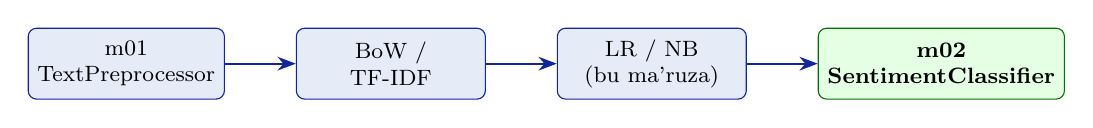
\begin{tikzpicture}[
      node distance=4mm and 9mm,
      box/.style={draw=cnublue,fill=cnubluebg,rounded corners=3pt,
                  minimum height=9mm,minimum width=24mm,
                  font=\footnotesize,align=center},
      goal/.style={draw=deepgreen,fill=green!10,rounded corners=3pt,
                   minimum height=9mm,minimum width=24mm,
                   font=\footnotesize\bfseries,align=center},
      arr/.style={-Stealth,cnublue,thick}
    ]
      \node[box]  (pre) {m01\\TextPreprocessor};
      \node[box,right=of pre] (vec) {BoW /\\TF-IDF};
      \node[box,right=of vec] (clf) {LR / NB\\(bu ma'ruza)};
      \node[goal,right=of clf](m02) {m02\\SentimentClassifier};
      \draw[arr] (pre)--(vec);
      \draw[arr] (vec)--(clf);
      \draw[arr] (clf)--(m02);
    \end{tikzpicture}
  \end{center}
  \vspace{4pt}
  \small P2 da qurasiz:
  \begin{itemize}
    \item \texttt{SentimentClassifier(m02)}:
          \texttt{fit()} / \texttt{predict()} / \texttt{predict\_proba()}
    \item LR va NB ni \texttt{macro $F_1$} bilan taqqoslash
    \item \texttt{confusion\_matrix} + \texttt{classification\_report}
  \end{itemize}
  \vspace{4pt}
  \begin{tcolorbox}[warnbox,title=P2 birinchi assert --- bu slayd [I2] dan]
    \footnotesize
    \texttt{assert abs(ratio - 3.375) < 0.01}\\
    \texttt{\# Ma'ruza L2 [I2]-slayd bilan solishtiring}
  \end{tcolorbox}
\end{frame}

% ----------------------------------------------------------------
% [R] ADABIYOTLAR
% ----------------------------------------------------------------
\begin{frame}{Adabiyotlar}
  \small
  \begin{enumerate}\setlength{\itemsep}{5pt}
    \item McCallum, A., Nigam, K.\ (1998).
          \textit{A Comparison of Event Models for Naive Bayes
          Text Classification.} AAAI/ICML-98 Workshop.

    \item Jurafsky, D., Martin, J.H.\ (2024).
          \textit{Speech and Language Processing}, 3rd ed.\
          \S4 (Naive Bayes), \S5 (Logistic Regression),
          \S4.7 (Evaluation).
          \textcolor{halfgray}{\footnotesize
            \texttt{web.stanford.edu/\textasciitilde jurafsky/slp3/}}

    \item Pedregosa, F.\ et al.\ (2011).
          Scikit-learn: Machine Learning in Python.
          \textit{JMLR} 12, 2825--2830.
          \textcolor{halfgray}{\footnotesize
            \texttt{sklearn.naive\_bayes},
            \texttt{sklearn.linear\_model},
            \texttt{sklearn.metrics}}

    \item Mitchell, M.\ et al.\ (2019).
          Model Cards for Model Reporting.
          \textit{FAccT~'19.}
          \textcolor{halfgray}{\footnotesize
            Etika va shaffoflik standarti.}
  \end{enumerate}
\end{frame}

% ================================================================
\appendix
% ================================================================

% ----------------------------------------------------------------
% [S1] SIGMOID MATEMATIK XOSSALARI
% ----------------------------------------------------------------
\begin{frame}{Ilova S1: Sigmoid Xossalari va Foydali Taxminlar}
  \small
  \textbf{Ta'rif:}\quad
  $\sigma(z)=\dfrac{1}{1+e^{-z}}$\\[6pt]
  \textbf{Hosila:}
  \[
    \sigma'(z)
    =\frac{e^{-z}}{(1+e^{-z})^2}
    =\sigma(z)\bigl(1-\sigma(z)\bigr)
  \]
  \textcolor{halfgray}{\footnotesize
    Isboti: $\tfrac{d}{dz}(1+e^{-z})^{-1}
    =(-1)(1+e^{-z})^{-2}(-e^{-z})=\tfrac{e^{-z}}{(1+e^{-z})^2}$}\\[5pt]
  \textbf{Chegaralar:}
  $\lim_{z\to+\infty}\sigma(z)=1$;\quad
  $\lim_{z\to-\infty}\sigma(z)=0$;\quad
  $\sigma(0)=0.5$\\[5pt]
  \textbf{Qo'lda hisob uchun taxminlar:}\\[3pt]
  $e^{-0.5}\approx 0.607$;\quad
  $e^{0.5}\approx 1.649$;\quad
  $e^{1.5}\approx 4.48$;\quad
  $e^{-1.5}\approx 0.223$;\quad
  $e^{1}\approx 2.718$
\end{frame}

% ----------------------------------------------------------------
% [S2] BAYES TEOREMI CHIQARISHI
% ----------------------------------------------------------------
\begin{frame}{Ilova S2: Bayes Teoremi Chiqarishi}
  \small
  \textbf{Birgalik ehtimollik:}
  \[
    P(y)\cdot P(\mathbf{x}\mid y)
    = P(y,\mathbf{x})
    = P(\mathbf{x})\cdot P(y\mid\mathbf{x})
  \]
  \textbf{Shundan:}
  \[
    P(y\mid\mathbf{x})
    =\frac{P(\mathbf{x}\mid y)\,P(y)}{P(\mathbf{x})}
  \]
  \textbf{Klassifikatsiyada:}
  $P(\mathbf{x})$ barcha $y$ lar uchun bir xil
  $\Rightarrow$ proporsional yozish mumkin:
  \[
    P(y\mid\mathbf{x})\;\propto\; P(\mathbf{x}\mid y)\,P(y)
  \]
  Shu sababli NB da maxraj ($P(\mathbf{x})$) hisoblash shart emas ---
  faqat numeratorlarni taqqoslaymiz.
\end{frame}

% ----------------------------------------------------------------
% [S3] F-BETA FORMULASI
% ----------------------------------------------------------------
\begin{frame}{Ilova S3: $F_\beta$ Formulasi}
  \small
  Agar Recall $R$ Precision $P$ dan muhimroq bo'lsa ($\beta>1$):
  \[
    F_\beta = \frac{(1+\beta^2)\,P\cdot R}{\beta^2\,P + R}
  \]
  \bunda{$\beta>1$: recallga ko'proq og'irlik;\quad
         $\beta<1$: precisionga ko'proq og'irlik}\\[6pt]
  \textbf{Misollar:}
  \begin{itemize}
    \item Tibbiy diagnoz: $\beta=2$ (FN juda qimmat)\\
          $F_2 = 5PR/(4P+R)$
    \item Spam filtri: $\beta=0.5$ (FP qimmat --- muhim xat yo'qolmasin)\\
          $F_{0.5} = 1.25PR/(0.25P+R)$
    \item Standart sentiment: $\beta=1$ $\Rightarrow$
          $F_1 = 2PR/(P+R)$
  \end{itemize}
\end{frame}

\end{document}
